\documentclass[11pt]{article}
\usepackage{graphicx}
\usepackage{titling}
\usepackage{array}
\newcolumntype{P}[1]{>{\centering\arraybackslash}p{#1}}
\newcolumntype{M}[1]{>{\centering\arraybackslash}m{#1}}
\setcounter{secnumdepth}{0}
\usepackage{caption}
\usepackage{geometry}
\geometry{
	top=2cm,
	left=2cm,
	right=2cm
}
\usepackage{hyperref}
\hypersetup{
	colorlinks=true,
	urlcolor=blue,
}
\urlstyle{same}

\tolerance=1
\emergencystretch=\maxdimen
\hyphenpenalty=10000
\hbadness=10000

\preauthor{%
  \begin{center}
  \LARGE
  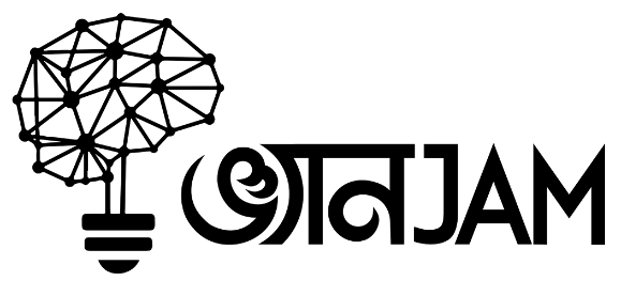
\includegraphics[scale=.4]{img/logo.png}\\[\bigskipamount]
}
\postauthor{\end{center}}
\title{Introduction to Machine Learning}
\date{}
\begin{document}
\maketitle
\section{Day 0}
Welcome to Machine Learning! Today you'll get yourself introduced with the idea of making a computer learn by itself without being explicitly programmed. You'll also see some classifications of Machine Learning problem, mainly:
\begin{itemize}
\item Supervised Learning
\begin{itemize}
\item Linear Regression
\item Logistic Regression
\item Linear Discriminant Analysis
\item K-Nearest Neighbors
\item Decision Trees
\end{itemize}
\item Unsupervised Learning
\begin{itemize}
\item K-Means Clustering
\item Principal Component Analysis
\item Anomaly Detection
\item Collaborative filtering and Recommender Systems
\end{itemize}
\item Reinfocement Learning
\end{itemize}
You can find the relevant materials for today in the links below:
\begin{itemize}
\item \href{https://www.youtube.com/watch?v=PPLop4L2eGk}{What Is Machine Learning}
\item \href{https://www.youtube.com/watch?v=bQI5uDxrFfA}{Supervised Learning}
\item \href{https://www.youtube.com/watch?v=jAA2g9ItoAc}{Unsupervised Learning}
\item \href{https://www.youtube.com/watch?v=JgvyzIkgxF0}{Reinforcement Learning}
\end{itemize}
\section{Day 1}
This day, you'll get to know the most widely used tools for Machine Learning that will speed up your Machine Learning algorithms with the help of cleverly optimized Linear Algebra libraries. This is possible because of a process called ``Vectorization'' which exploits the benefits of SIMD (Single Intruction Multiple Data) Parallelism, which speeds up your algorithms by a factor of ~ 400-600. Mainly, the tools that you'll be using through this course are:
\begin{itemize}
\item Python\\
There are some linear algebra libraries of python that you'll get accustomed to throughout this course.
\begin{itemize}
\item SciPy
\item NumPy
\item Matplotlib
\end{itemize}
\item JupyterLab
\item Conda
\item Examples of Data Visualization using Matplotlib
\item Basic Linear Algebra for Machine Learning
\end{itemize}
\begin{center}
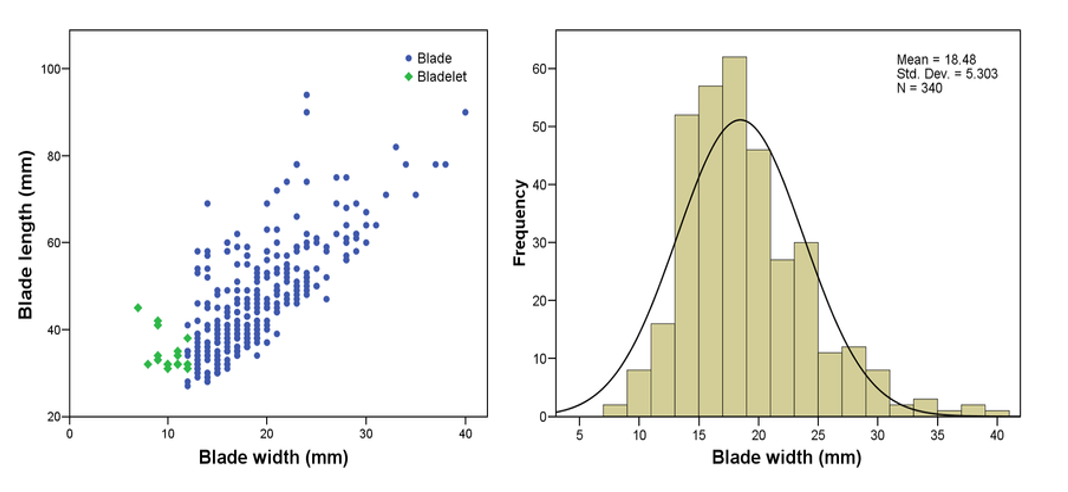
\includegraphics[scale=.7]{img/dataVis.png}
\end{center}
There are some links that you will need to visit frequently while exercising ML algorithms, and these are listed below for your convenience:
\begin{itemize}
\item \href{https://numpy.org/doc/stable/}{Numpy} Documentation
\item \href{https://matplotlib.org/contents.html}{Matplotlib} Documentation
\item \href{https://www.python.org/doc/}{Python} Documentation
\item \href{https://jupyterlab.readthedocs.io/en/stable/}{JupyterLab} Documentation
\item \href{https://www.youtube.com/watch?v=23aQdrS58e0}{Conda} Introduction
\end{itemize}
\pagebreak
\section{Day 2}
Today you will learn basic Linear Regression and Gradient Descent, as well as some optimization for your learning algorithms including Feature Scaling and Mean Normalization. You'll need to have a brief idea of basic differential calculus for Gradient Descent as a pre-requisite. Using Linear Regression and Gradient Descent, you can fit a linear model on a sample dataset as follows:\\
\begin{center}
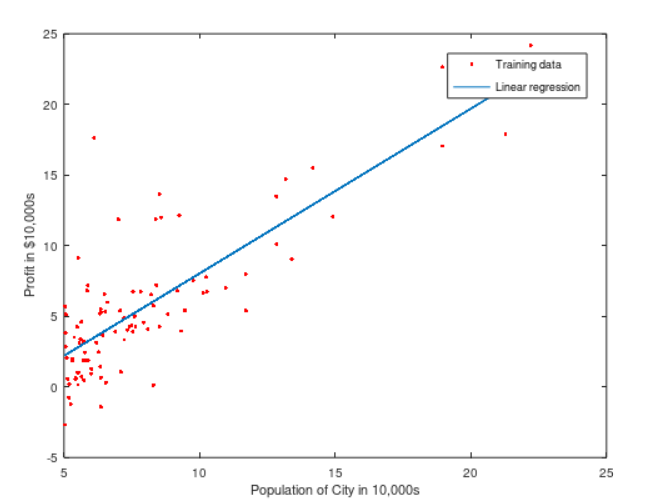
\includegraphics[scale=.7]{img/simplifiedGd.png}
\end{center}
List of relevant information and videos:
\begin{itemize}
\item \href{https://www.youtube.com/watch?v=kHwlB_j7Hkc}{Representing the model}
\item \href{https://www.youtube.com/watch?v=yuH4iRcggMw}{Squared error cost function}
\item \href{https://www.youtube.com/watch?v=e1nTgoDI_m8}{Feature scaling and Mean normalization}
\item \href{https://www.youtube.com/watch?v=YovTqTY-PYY}{Gradient Descent}
\end{itemize}
\pagebreak
\section{Day 3}
Logistic regression is a classification algorithm. Unlike regression algorithms which gives a continuous valued output, classification algorithms provide discrete valued output which can be used for creating decision boundaries and digit recognition.\\ 
\begin{center}
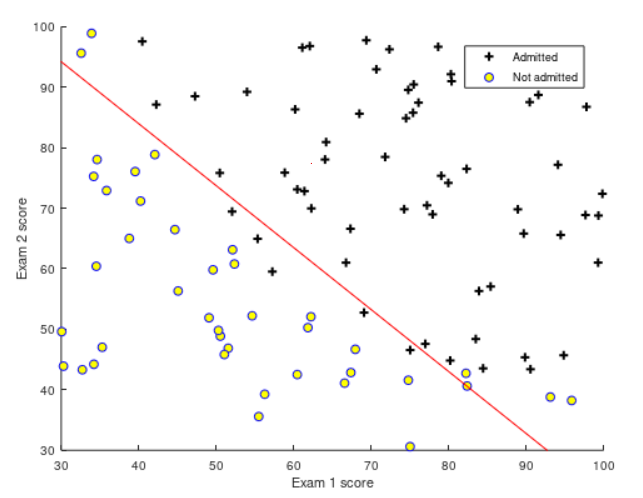
\includegraphics[scale=.7]{img/simplifiedLogReg}
\end{center}
Further optimizing the learning algorithms by using multiple features can be used to find out non-linear decision boundaries.
\begin{center}
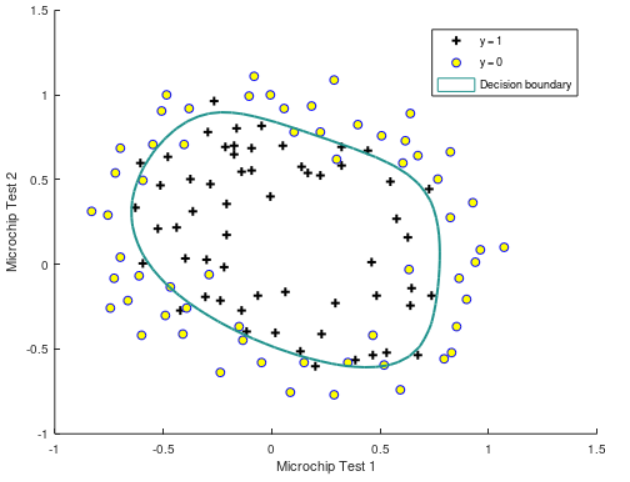
\includegraphics[scale=.7]{img/simplifiedRegLogReg.png}
\end{center}
\begin{itemize}
\item \href{https://www.youtube.com/watch?v=t1IT5hZfS48}{Logistic Regression concept}
\item \href{https://www.youtube.com/watch?v=F_VG4LNjZZ}{Decision boundary}
\item \href{https://www.youtube.com/watch?v=HIQlmHxI6-0}{Cost function for Logistic regression}
\item \href{https://www.youtube.com/watch?v=ISBGFY-gBug}{Bias and Variance}
\item \href{https://www.youtube.com/watch?v=KvtGD37Rm5I}{Regularization}
\end{itemize}
\section{Day 4}
More supervised learning algorithms will give you a brief overview of Linear Discriminant Analysis, K-Nearest Neighbors and Decision trees. 
\begin{figure}[h!]
\begin{center}
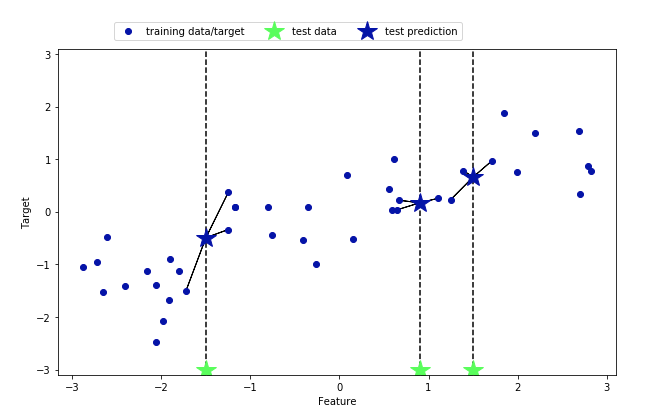
\includegraphics[scale=.5]{img/knn2.png}
\end{center}
{\caption*{K-Nearest Neighbors}}
\begin{center}
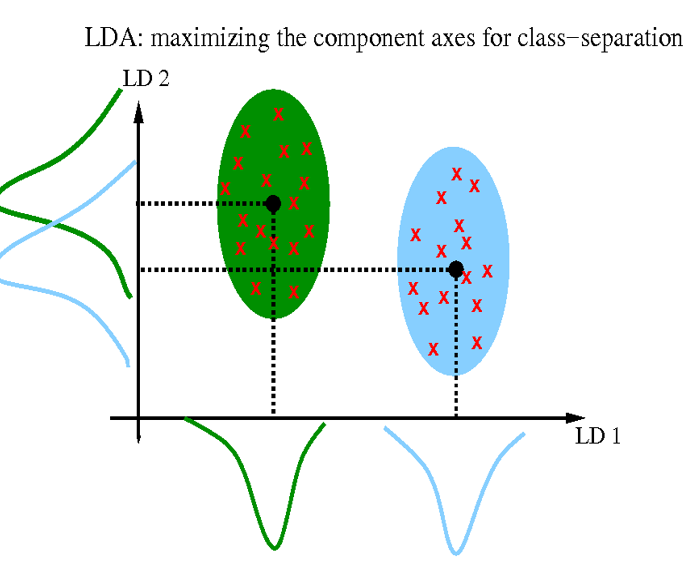
\includegraphics[scale=.6]{img/lda.png}
\end{center}
\end{figure}
\begin{itemize}
\item \href{https://www.youtube.com/watch?v=HVXime0nQeI}{K-Nearest Neighbors}
\item \href{https://www.youtube.com/watch?v=azXCzI57Yfc}{Linear Discriminant Analysis}
\item \href{https://www.youtube.com/watch?v=7VeUPuFGJHk}{Decision Trees}
\end{itemize}
\end{document}





















